\section{Topologies}
    When one uses the notation developed for intervals on the real line $[a,b]$
    and $(a,b)$, the former is called the \textit{closed} interval and the
    latter the \textit{open} interval. The clearest difference is that $[a,b]$
    has it's endpoints, whereas $(a,b)$ does not. We can generalize this
    further. For every point $x\in(a,b)$ there is some $\varepsilon>0$ such that
    we can fit $(x-\varepsilon,x+\varepsilon)$ inside of the interval $(a,b)$.
    Namely, define $\varepsilon$ to be:
    \begin{equation}
        \varepsilon=\frac{\min\{b-x,x-a\}}{2}
    \end{equation}
    From this we have $(x-\varepsilon,x+\varepsilon)\subseteq(a,b)$
    (Fig.~\ref{fig:Open_Interval_is_Open_Subset_of_R}).
    \begin{figure}[H]
        \centering
        \captionsetup{type=figure}
        \begin{tikzpicture}[>=Latex]
    \coordinate (a)  at (2.0,  0.0);
    \coordinate (b)  at (9.0,  0.0);
    \coordinate (xt) at (4.0,  0.1);
    \coordinate (xb) at (4.0, -0.1);
    \coordinate (x)  at (4.0,  0.0);
    \coordinate (xl) at (3.0,  0.0);
    \coordinate (xr) at (5.0,  0.0);

    \draw[<->]   (0, 0) to (10, 0) node[above] {$\mathbb{R}$};
    \draw[thick] (a) to (b);
    \draw[thick] (b) arc (0:15:0.5);
    \draw[thick] (b) arc (0:-15:0.5);
    \draw[thick] (a) arc (180:195:0.5);
    \draw[thick] (a) arc (180:165:0.5);

    \draw (xt) to (xb);

    \node at (a)  [below=1ex] {$a$};
    \node at (b)  [below=1ex] {$b$};
    \node at (xl) [below=1ex] {$x-\varepsilon$};
    \node at (xr) [below=1ex] {$x+\varepsilon$};
    \node at (x)  [below=1ex] {$x$};

    \draw[blue, thick] (xr) arc (0:15:0.5);
    \draw[blue, thick] (xr) arc (0:-15:0.5);
    \draw[blue, thick] (xl) arc (180:195:0.5);
    \draw[blue, thick] (xl) arc (180:165:0.5);
    \draw[blue, thick] (xr) to (xl);
\end{tikzpicture}
        \caption{The Open Interval $(a,b)$ is an Open Subset of $\mathbb{R}$}
        \label{fig:Open_Interval_is_Open_Subset_of_R}
    \end{figure}
    This cannot be done for the closed unit interval. If we let $x=a$, then for
    any $\varepsilon>0$ we have that $(a-\varepsilon,a+\varepsilon)$ has points
    that fall outside of $[a,b]$. That is, all of the points between
    $a-\varepsilon$ and $a$ (Fig.~\ref{fig:Closed_Interval_is_Not_Open}).
    This is the distinction we want to note between a closed interval
    and an open interval, and we wish to axiomatize these properties.
    \begin{figure}[H]
        \centering
        \captionsetup{type=figure}
        \begin{tikzpicture}[>=Latex]
    % Coordinates for various points.
    \coordinate (a)  at (4.0,  0.0);
    \coordinate (b)  at (9.0,  0.0);
    \coordinate (xl) at (3.0,  0.0);
    \coordinate (xr) at (5.0,  0.0);

    % Draw the real line.
    \draw[<->]   (0, 0) to (10, 0) node[above] {$\mathbb{R}$};

    % Draw the closed interval [a, b].
    \draw[thick] (a) to (b);

    % Add "brackets" indicating it is a closed interval.
    \draw[thick] (8.9, 0.1) to (9.0, 0.1) to (9.0, -0.1) to (8.9, -0.1);
    \draw[thick] (4.1, 0.1) to (4.0, 0.1) to (4.0, -0.1) to (4.1, -0.1);

    % Labels for the vaious points.
    \node at (a)  [below=1ex] {$a$};
    \node at (b)  [below=1ex] {$b$};
    \node at (xl) [below=1ex] {$a-\varepsilon$};
    \node at (xr) [below=1ex] {$a+\varepsilon$};

    % Draw the part of the open interval (a-e, a+e) that is inside of [a, b].
    \draw[blue, thick] (xr) arc (0:15:0.5);
    \draw[blue, thick] (xr) arc (0:-15:0.5);
    \draw[blue, thick] (a) to (xr);

    % Draw the part that falls outside.
    \draw[red, thick]  (xl) arc (180:195:0.5);
    \draw[red, thick]  (xl) arc (180:165:0.5);
    \draw[red, thick]  (a) to (xl);
\end{tikzpicture}
        \caption{The Closed Interval $[a,b]$ is Not Open.}
        \label{fig:Closed_Interval_is_Not_Open}
    \end{figure}
    If we take the intersection of two intervals $(a,b)$ and $(c,d)$, then the
    result is either the empty set or it is once again an open interval. More
    importantly, if the intersection is non-empty then we can find an
    $\varepsilon>0$ such that $(x-\varepsilon,x+\varepsilon)$ fits inside the
    intersection. That is, letting $\varepsilon_{1}$ and $\varepsilon_{2}$ be
    such that $(x-\varepsilon_{1},x+\varepsilon_{1})\subseteq(a,b)$ and
    $(x-\varepsilon_{2},x+\varepsilon_{2})\subseteq(c,d)$, taking
    $\varepsilon=\min\{\varepsilon_{1},\varepsilon_{2}\}$ gives us the desired
    result. This is our first \textit{axiom}: Topologies should be closed to
    the intersection of open sets (see Fig.). Since the intersection of
    $(a,b)$ and $(c,d)$ may be empty, we must consider the empty set $\emptyset$
    to be a member of the topology as well.
    \begin{figure}[H]
        \centering
        \captionsetup{type=figure}
        \begin{tikzpicture}[>=Latex]
    \coordinate (a)  at (2.0,  0.0);
    \coordinate (b)  at (7.0,  0.0);
    \coordinate (c)  at (3.0,  0.0);
    \coordinate (d)  at (9.0,  0.0);
    \coordinate (x)  at (5.0,  0.0);
    \coordinate (xb) at (5.0, -0.1);
    \coordinate (xt) at (5.0,  0.1);
    \coordinate (xl) at (4.2,  0.0);
    \coordinate (xr) at (5.8,  0.0);

    \draw[<->]   (0, 0) to (10, 0) node[above] {$\mathbb{R}$};

    \node at (a)  [below=1ex] {$a$};
    \node at (b)  [below=1ex] {$b$};
    \node at (c)  [below=1ex] {$c$};
    \node at (d)  [below=1ex] {$d$};
    \node at (xl) [below=1ex] {$x-\varepsilon$};
    \node at (xr) [below=1ex] {$x+\varepsilon$};
    \node at (x)  [below=1ex] {$x$};
    \node at (a)  [above=1ex]
        {$\color{blue}{(a,b)}\cap\color{red}{(c,d)}=\color{Violet}{(c,b)}$};
    \node at (b) [above=1ex]
        {$\color{cyan}{(x-\varepsilon,x+\varepsilon)}%
            \subseteq\color{Violet}{(c,b)}$};

    \draw[blue,   thick]    (a)  to (c);
    \draw[red,    thick]    (b)  to (d);
    \draw[Violet, thick]    (c)  to (xl);
    \draw[Violet, thick]    (xr) to (b);
    \draw[cyan, very thick] (xl) to (xr);

    \draw[thin] (xt) to (xb);

    \draw[blue, very thick] (b) arc (0:15:0.5);
    \draw[blue, very thick] (b) arc (0:-15:0.5);
    \draw[blue, very thick] (a) arc (180:195:0.5);
    \draw[blue, very thick] (a) arc (180:165:0.5);

    \draw[red, very thick] (d) arc (0:15:0.5);
    \draw[red, very thick] (d) arc (0:-15:0.5);
    \draw[red, very thick] (c) arc (180:195:0.5);
    \draw[red, very thick] (c) arc (180:165:0.5);

    \draw[cyan, very thick] (xr) arc (0:15:0.5);
    \draw[cyan, very thick] (xr) arc (0:-15:0.5);
    \draw[cyan, very thick] (xl) arc (180:195:0.5);
    \draw[cyan, very thick] (xl) arc (180:165:0.5);
\end{tikzpicture}
        \caption{The Intersection of Open Intervals is Open.}
        \label{fig:Closed_Interval_is_Not_Open}
    \end{figure}
    Lastly,
    if we take the union over an arbitrary collection of open intervals, then
    end result may not be an open interval, but it will still have the property
    that for any $x$ in the union there is a $\varepsilon>0$ such that
    $(x-\varepsilon,x+\varepsilon)$ fits inside the union. This is the property
    we will ascribe to \textit{open}\index{Open Set} subsets of $\mathbb{R}$:
    an open subset of $\mathbb{R}$ is a set $\mathcal{U}\subseteq\mathbb{R}$
    such that for all $x\in\mathcal{U}$ there is an $\varepsilon>0$ such that
    $(x-\varepsilon,x+\varepsilon)\subseteq\mathcal{U}$. It is these two
    properties of open sets that we wish to capture: Closure to finite
    intersections and arbitrary unions. We've already noted that the
    intersection of two open intervals may be empty, and so we want to claim
    that the empty set is open as well. Lastly, we may regard the entire real
    line $\mathbb{R}$ as the \textit{interval} $(\minus\infty,\infty)$, and
    because of this we wish to regard all of $\mathbb{R}$ to be open too. In
    generalizing these notions we can define a \textit{topology} on a set $X$.
    \begin{fdefinition}{Topology}{Topology}
        A \gls{topology} on a \gls{set} $X$ is a \gls{subset}
        $\tau\subseteq\mathcal{P}(X)$ such that $\emptyset\in\tau$, $X\in\tau$,
        and for any subset $\mathcal{O}\subseteq\tau$, it is true that:
        \begin{equation*}
            \bigcup_{\mathcal{U}\in\mathcal{O}}\mathcal{U}\in\tau
        \end{equation*}
        And such that for all $A,B\in\tau$, it is true that $A\cap{B}\in\tau$.
    \end{fdefinition}
    There are many trivial examples of topologies on any set $X$, but the
    trivial examples often provide excellent counterexamples for various
    propositions. The two extreme topologies are the \textit{discrete} topology
    and the \textit{chaotic} topology. The chaotic topology is also called the
    trivial topology or the indiscrete topology.\index{Trivial Topology}%
    \index{Indiscrete Topology}\index{Chaotic Topology}\index{Topology!Trivial}%
    \index{Topology!Chaotic}\index{Topology!Indiscrete}\index{Topology!Discrete}
    \begin{theorem}
        \label{thm:discrete_topology_is_a_topology}%
        If $X$ is a set, the $\mathcal{P}(X)$ is a topology on $X$.
        \index{Discrete Topology}
    \end{theorem}
    \begin{proof}
        For $\emptyset\subseteq{X}$ (Thm.~\ref{thm:Emptyset_Is_Subset}) and
        $X\subseteq{X}$ (Thm.~\ref{thm:Reflexivity_of_Inclusion}), and thus it
        is true that $\emptyset\in\mathcal{P}(X)$ and $X\in\mathcal{P}(X)$
        (Def.~\ref{def:Power_Set}). If $\mathcal{O}\subseteq\mathcal{P}(X)$,
        then $\bigcup\mathcal{O}\subseteq{X}$ (Def.~\ref{def:Union_over_a_Set}).
        Lastly, if $A,B\in\mathcal{P}(X)$, then $A\subseteq{X}$ and
        $B\subseteq{X}$, and thus $A\cap{B}\subseteq{X}$
        (Thm.~\ref{thm:Intersection_of_Subsets_is_Still_Subset}). Thus,
        $\mathcal{P}(X)$ is a topology on $X$ (Def.~\ref{def:Topology}).
    \end{proof}
    \begin{theorem}
        \label{thm:chaotic_topology_is_topology}%
        If $X$ is a set, then $\{\emptyset,X\}$ is a topology on $X$.
    \end{theorem}
    \begin{proof}
        For by definition $\emptyset\in\{\emptyset\}$ and $X\in\{\emptyset,X\}$
        (Thm.~\ref{thm:Existence_of_Set_Built_from_Two_Sets}). If
        $\mathcal{O}\subseteq\{\emptyset,X\}$, then by the law of the excluded
        middle either $X\in\mathcal{O}$ or $X\notin\mathcal{O}$. If
        $X\in\mathcal{O}$, then $\bigcup\mathcal{O}=X$, and if not, then
        $\bigcup\mathcal{O}=\emptyset$. In either case,
        $\bigcup\mathcal{O}\in\{\emptyset,X\}$. If $A,B\in\{\emptyset,X\}$, then
        either one of these is the empty set or not. If so, then
        $A\cap{B}=\emptyset$ (Thm.~\ref{thm:Intersection_with_Emptyset}), and
        if not then $A=X$ and $B=X$, and thus $A\cap{B}=X$
        (Thm.~\ref{thm:Idempotent_Law_of_Intersections}). Thus,
        $A\cap{B}\in\{\emptyset,X\}$, and $\{\emptyset,X\}$ is a topology on $X$
        (Def.~\ref{def:Topology}).
    \end{proof}
    \begin{example}
        The Discrete Topology\index{Discrete Topology}\index{Discrete!Topology}
        on a set $X$ is simply $\tau=\mathcal{P}(X)$. That is, the
        \gls{power set}\index{Power Set} of $X$. This is indeed a topology as
        proved in Thm.~\ref{thm:discrete_topology_is_a_topology}. Since a
        topology is a subset of $\mathcal{P}(X)$ (by definition), the discrete
        topology is thus the \textit{largest} topology that one can consider on
        a given set. It is called the discrete topology since it arises from the
        \textit{discrete metric}\index{Discrete!Metric}. This metric, which is
        of great importance to the theory of \textit{metric spaces}%
        \index{Metric Space}, defines a fairly trivial distance between all of
        the points in $X$. If $x,y\in{X}$ and $x=y$, the distance is
        $d(x,y)=0$. If $x\ne{y}$, then $d(x,y)=1$. The topology
        \textit{generated}\index{Topology!Induced by Metric} from this metric
        is precisely the discrete topology $\mathcal{P}(X)$. One of the strange
        properties of the discrete topology is that any function
        $f:X\rightarrow{A}$ is \textit{continuous} (to be defined)%
        \index{Function!Continuous}\index{Continuous Function}
        regardless of the topology on $A$.
    \end{example}
    \begin{example}
        The chaotic topology\index{Chaotic Topology} is $\tau=\{\emptyset,X\}$.
        This is also a topology, as demonstrated in
        Thm.~\ref{thm:chaotic_topology_is_topology}, but we can also check this
        by simple computation. The empty set and the whole space are contained
        within $\tau$, and there are only four possible ways to perform unions
        and intersections. The commutativity of union and intersection reduces
        this to three. We have:
        \par
        \begin{subequations}
            \begin{minipage}[b]{0.49\textwidth}
                \begin{align}
                    \emptyset\cap\emptyset&=\emptyset\\
                    \emptyset\cap{X}&=\emptyset\\
                    X\cap{X}&=X
                \end{align}
            \end{minipage}
            \hfill
            \begin{minipage}[b]{0.49\textwidth}
                \begin{align}
                    \emptyset\cup\emptyset&=\emptyset\\
                    \emptyset\cup{X}&=X\\
                    X\cup{X}&=X
                \end{align}
            \end{minipage}
        \end{subequations}
        \par\vspace{2.5ex}
        The chaotic topology is so named for one of it's strange properties. As
        we will see once we've defined continuity, the chaotic topology has the
        property that every single function $f:A\rightarrow{X}$ will be
        continuous, regardless of what the topology chosen on $A$ was. Unlike
        the discrete topology, the chaotic topology is almost never associated
        with a metric space. Indeed, the chaotic space is induced from a metric
        if and only if $X$ has one point (in which case it is equivalent to
        the discrete topology).
    \end{example}
    \begin{example}
        The Sierpinski topology\index{Sierpinski Topology} is a topology placed
        on $\mathbb{Z}_{2}=\{0,1\}$. It is defined as the set:
        \begin{equation}
            \tau_{S}=\{\,\emptyset,\,\{0\},\,\mathbb{Z}_{2}\,\}
        \end{equation}
        By definition $\tau_{S}$ contains both the empty set and the entirety of
        $\mathbb{Z}_{2}$. Checking unions is trivial since
        $\emptyset\subseteq\{0\}\subseteq\mathbb{Z}_{2}$, and thus any union of
        any collection $\mathcal{O}\subseteq\tau_{S}$ is simply the
        \textit{largest} set in the collection, meaning $\tau_{S}$ is closed to
        arbitrary unions. Moreover, all of the intersections are trivial:
        If $A=\emptyset$, then $A\cap{B}=\emptyset$, if $A=\mathbb{Z}_{2}$, then
        $A\cap{B}=B$, and lastly if $A=\{0\}$ and $B=\{0\}$, then
        $A\cap{B}=\{0\}$ meaning $\tau_{S}$ is closed to finite intersections.
        Hence, it is a topology (Def.~\ref{def:Topology}). This too serves as a
        test case for many plausible propositions.
    \end{example}
    \begin{figure}[H]
        \centering
        \captionsetup{type=figure}
        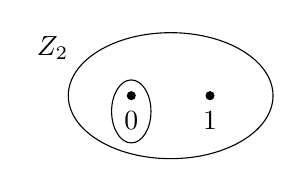
\begin{tikzpicture}
    \draw (0, 0) circle (1.3cm and 0.8cm);
    \draw (-0.5, -0.2) circle (0.25cm and 0.4cm);
    \draw[fill=black] (-0.5, 0.0) circle (0.5mm) node[below=0.5ex] {$0$};
    \draw[fill=black] ( 0.5, 0.0) circle (0.5mm) node[below=0.5ex] {$1$};
    \node at (-1.5, 0.6) {$\mathbb{Z}_{2}$};
\end{tikzpicture}
        \caption{The Sierpinski Topology}
        \label{fig:Sierpinksi_Topology}
    \end{figure}
    We can be a little more general, defining a Sierpinski-like topology on any
    non-empty set.
    \begin{theorem}
        \label{thm:Existence_of_Sierpinski_Like_Topology}%
        If $X$ is a non-empty set and if $x\in{X}$, then the set $\tau$ defined
        by $\tau=\{\emptyset,\{x\},X\}$ is a topology on $X$.
    \end{theorem}
    \begin{proof}
        For $\emptyset,X\in\tau$. If $\mathcal{O}\subseteq\tau$, either
        $X\in\mathcal{O}$ or $X\notin\mathcal{O}$. If $X\in\mathcal{O}$, then
        $\bigcup\mathcal{O}=X$, which is contained in $\tau$. If
        $X\notin\mathcal{O}$, either $\{x\}\in\mathcal{O}$ or not. If
        $\{x\}\in\mathcal{O}$, then $\bigcup\mathcal{O}=\{x\}$, which is
        contained in $\tau$. Lastly, if neither $X$ nor $\{x\}$ are elements of
        $\mathcal{O}$, then either $\mathcal{O}=\emptyset$ or
        $\mathcal{O}=\{\emptyset\}$. In either case,
        $\bigcup\mathcal{O}=\emptyset$. Thus, $\tau$ is closed to arbitrary
        unions. Similarly, if $A,B\in\tau$, and if either $A$ or $B$ are empty,
        then $A\cap{B}=\emptyset$. If neither $A$ nor $B$ are empty, then
        either $A$ or $B$ is the set $\{x\}$, or both are the whole space. In
        the former case $A\cap{B}=\{x\}$ and in the latter $A\cap{B}=X$. In
        both scenarios the intersection is contained in $\tau$. Hence,
        $\tau$ is a topology on $X$ (Def.~\ref{def:Topology}).
    \end{proof}
    If $X$ is a single point, $X=\{x\}$, then the Sierpinski-like topology
    defined in Thm.~\ref{thm:Existence_of_Sierpinski_Like_Topology} is simply
    the chaotic topology, which is also the discrete topology on one point.
    This is because, since $\{x\}=X$, the set $\{\emptyset,\{x\},X\}$ is equal
    to the set $\{\emptyset,X\}$ (recall that sets have no notion of
    repetition). A further generalization goes as follows:
    \begin{theorem}
        \label{thm:Existence_of_Generalized_Sierpinski_Like_Topology}
        If $X$ is a set, if $\mathcal{U}\subseteq{X}$, and if
        $\tau=\{\emptyset,\mathcal{U},X\}$, then $\tau$ is a topology
        on $X$.
    \end{theorem}
    \begin{proof}
        For $\emptyset,X\in\tau$. If $\mathcal{O}\subset\tau$, either
        $X\in\mathcal{O}$ or not. If it is, then $\bigcup\mathcal{O}=X$.
        If not, then either $\mathcal{U}\in\mathcal{O}$ or not. If it is,
        then $\bigcup\mathcal{O}=\mathcal{U}$. If not, then
        $\bigcup\mathcal{O}=\emptyset$. In any of the three cases, the union is
        contained in $\tau$ and so we have closure with respect to arbitrary
        unions. Similarly, it is closed to intersections, and is therefore a
        topology (Def.~\ref{def:Topology}).
    \end{proof}
    A set combined with a topology on it is called a topological space. These
    are the main objects, together with continuous functions, of study in
    topology.
    \begin{fdefinition}{Topological Space}{Topological_Space}
        A \gls{topological space}, denote $(X,\tau)$ is a \gls{set} $X$ and a
        \gls{topology} $\tau$ on $X$.
    \end{fdefinition}
    We pause to briefly digress about metric spaces, which are the most
    important example of topological spaces. Metric spaces are spaces which
    generalize the notion of \textit{distance} in Euclidean space%
    \index{Metric Space}\index{Euclidean Space}. These were first introduced by
    Maurice Fr\'{e}chet in 1906, and were the primary motivator for developing
    point-set topology in detail. A \textit{metric}\index{Metric} on a set $X$
    is a function $d:X\times{X}\rightarrow\mathbb{R}$ with the following four
    properties:
    \begin{align}
        d(x,y)&\geq{0}
        \tag{Positivity}\\
        d(x,y)&=0\Longrightarrow{x=y}
        \tag{Definiteness}\\
        d(x,y)&=d(y,x)
        \tag{Symmetry}\\
        d(x,z)\leq{d}(x,y)+d(y,z)
        \tag{Triangle Inequality}
    \end{align}
    The problem of proving whether or not a given function is a metric is eased
    slightly since symmetry can be proved from definiteness and the triangle
    inequality. As stated before, this is a generalization of the notion of
    distance, and as such the primary examples come from Euclidean space. In
    $\mathbb{R}$ the distance function is the \textit{absolute value} function:
    $d(x,y)=|x-y|$. In higher dimension, $\mathbb{R}^{n}$, we use the
    Pythagorean theorem\index{Pythagoras' Theorem} to define distance:
    \begin{equation}
        d(\mathbf{x},\mathbf{y})
        =\sqrt{\sum_{k\in\mathbb{Z}_{n}}(x_{k}-y_{k})^{2}}
    \end{equation}
    A subset $\mathcal{U}$ of a metric space $(X,d)$ is called
    \textit{metrically open} if for all $x\in\mathcal{U}$ there is an
    $\varepsilon>0$ such that, for all $y\in{X}$ such that $d(x,y)<\varepsilon$,
    it is true that $y\in\mathcal{U}$. The collection of all metrically open
    subsets of a metric space form a topology on $X$, and this is called the
    topology induced by the metric\index{Topology!Induced by Metric}. Metric
    spaces are extremely well-behaved spaces and many theorems in topology are
    dedicated to proving that certain topological spaces can be given
    compatible metrics.
    \par\hfill\par
    There are two common ways in which to teach point-set topology: start with
    metric spaces or end with them. Starting with them is the pedagogical
    choice, since they are intuitive and any student who has taken a course in
    real analysis should have no problem solving problems about such spaces. The
    logical route is to end with them, since many of the fundamental theorems
    about metric spaces become short corollaries when one has developed a
    sufficient amount of topology. We will adopt the latter option, saving
    metric spaces for after we've developed connectedness, compactness, and the
    plethora of other \textit{topological} concepts (concepts that do not need
    a notion of distance, just a topology). An attempt will be made to give
    intuition in the form of examples, usually with Euclidean spaces or by
    presenting pictures. It is hoped that the abstraction will not be too
    confusing, but the end result is well worth it. Indeed, theorems such as the
    \textit{intermediate value theorem} and the \textit{extreme value theorem}
    from calculus can be proven in just a few lines once one has the right
    tools.
    \par\hfill\par
    One of the common problems in analysis, geometry, and topology is placing a
    \textit{natural} topology on a given set. That is, some how concocting an
    \textit{obvious} or most useful topology. The construction often goes by
    considering the smallest topology that has a certain property, smallest
    meaning the intersection of all other topologies with said property. It
    would be essential, then, to know that the intersection of topologies is
    again a topology. We prove this now.
    \begin{ltheorem}{The Intersection of Topologies is a Topology}
                   {Intersection_of_Topologies_is_a_Topology}
        If $X$ is a set, if $\Omega$ is a non-empty set such that for all
        $\tau\in\Omega$ it is true that $\tau$ is a topology on $X$, then
        $\bigcap\Omega$ is a topology on $X$.
    \end{ltheorem}
    \begin{proof}
        For since $\Omega$ is non-empty there is a set $\tau\in\Omega$
        (Def.~\ref{def:Non_Empty_Set}). But by hypothesis, if $\tau\in\Omega$
        then $\tau$ is a topology on $X$, and thus $\emptyset,X\in\tau$.
        Suppose $\emptyset\notin\bigcap\Omega$. Then there exists
        $\xi\in\Omega$, $\xi\ne\tau$, such that $X\notin\xi$
        (Def.~\ref{def:Intersection_Over_a_Collection}). But if $\xi\in\Omega$
        then $\xi$ is a topology on $X$, and thus $X\in\xi$
        (Def.~\ref{def:Topology}), thus $X\in\xi$, and similarly
        $\emptyset\in\xi$. Suppose there is an
        $\mathcal{O}\subseteq\bigcap\Omega$ such that
        $\bigcup\mathcal{O}\notin\bigcap\Omega$. But for all
        $\mathcal{U}\in\mathcal{O}$ it is true that
        $\mathcal{U}\in\bigcap\Omega$ since $\mathcal{O}$ is a subset of
        $\bigcap\Omega$ (Def.~\ref{def:Subsets}). But then for all
        $\tau\in\bigcap\Omega$ is it true that $\mathcal{U}\in\tau$
        (Def.~\ref{def:Intersection_Over_a_Collection}). But $\tau$ is a
        topology on $X$, and thus $\bigcup\mathcal{O}\in\tau$
        (Def.~\ref{def:Topology}). And this is true of all such $\tau$, and thus
        $\bigcup\mathcal{O}\in\bigcap\Omega$, a contradiction. Thus
        $\bigcap\Omega$ is closed to arbitrary unions. Lastly, if
        $A,B\in\bigcap\Omega$, then for all $\tau\in\bigcap\Omega$ it is true
        that $A,B\in\tau$. But $\tau$ is a topology, and thus
        $A\cap{B}\in\tau$ (Def.~\ref{def:Topology}). And since this is true of
        all $\tau\in\bigcap\Omega$, it is true that $A\cap{B}\in\bigcap\Omega$
        (Def.~\ref{def:Intersection_Over_a_Collection}). Therefore
        $\bigcap\Omega$ is a topology on $X$ (Def.~\ref{def:Topology}).
    \end{proof}
    \begin{figure}[H]
        \centering
        \captionsetup{type=figure}
        \begin{tikzpicture}[>=Latex]
    \draw[<->] (-3,  0) to (3, 0);
    \draw[<->] ( 0, -3) to (0, 3);
    \draw[fill=blue!70!white, densely dashed, opacity=0.6]
        (1, -1) to[out=90,  in=0]   (0, -0.5) to[out=180, in=-90] (-1, 0)
                to[out=90,  in=180] (0,  0.5) to[out=0,   in=-90] ( 1, 1) 
                to[out=90,  in=0]   (0,  1.5) to[out=180, in=90]  (-2, 0)
                to[out=-90, in=180] (0, -1.5) to[out=0, in=-90]   cycle;
    \draw[fill=red!70!white, densely dashed, opacity=0.6]
        (-1, -1) to[out=90,  in=180] (0, -0.5) to[out=0, in=-90]     ( 1, 0)
                 to[out=90,  in=0]   (0,  0.5) to[out=180,   in=-90] (-1, 1) 
                 to[out=90,  in=180] (0,  1.5) to[out=0, in=90]      ( 2, 0)
                 to[out=-90, in=0]   (0, -1.5) to[out=180, in=-90]   cycle;
    \node at (-2, 1) {$\color{blue!70!white}{\mathcal{U}_{1}}$};
    \node at ( 2, 1) {$\color{red!70!white}{\mathcal{U}_{2}}$};
    \node at ( 2, 2) {$\mathbb{R}^{2}$};
\end{tikzpicture}
        \caption{The Union of Topologies Need Not be Closed
                 to Finite Intersections}
        \label{fig:Union_of_Topologies_Not_Closed_to_Intersections}
    \end{figure}
    However, the union of topologies may not be a topology. For consider the two
    Sierpinski-like topologies on $\mathbb{Z}_{3}$ defined by
    $\tau_{1}=\{\emptyset,\{0\},\mathbb{Z}_{3}\}$ and
    $\tau_{2}=\{\emptyset,\{1\},\mathbb{Z}_{3}\}$. Both of these are topologies,
    however $\tau_{1}\cup\tau_{2}=\{\emptyset,\{0\},\{1\},\mathbb{Z}_{3}\}$,
    which is not a topology since it is not closed to unions. Note that
    $\{0\}\in\tau_{1}\cup\tau_{2}$, as is the set $\{1\}$, however $\{0,1\}$ is
    not. This is why we chose $\mathbb{Z}_{3}$ for our counterexample. Picking
    $\mathbb{Z}_{2}$ would actually result in a topology since
    $\{0,1\}=\mathbb{Z}_{2}$, and the whole space would be contained in the
    union. Thus we see that the union of topologies may not be closed to
    arbitrary unions, but it need not be closed to intersections either.
    Consider the topologies on $\mathbb{R}^{2}$ defined by
    $\tau_{1}=\{\emptyset,\mathcal{U}_{1},\mathbb{R}^{2}\}$ and
    $\tau_{2}=\{\emptyset,\mathcal{U}_{2},\mathbb{R}^{2}\}$, where
    $\mathcal{U}_{1}$ and $\mathcal{U}_{2}$ are the two blobs shown in
    Fig.~\ref{fig:Union_of_Topologies_Not_Closed_to_Intersections}. Since
    $\mathcal{U}_{1}\subseteq\mathbb{R}^{2}$, as well as
    $\mathcal{U}_{2}\subseteq\mathbb{R}^{2}$, by
    Thm.~\ref{thm:Existence_of_Generalized_Sierpinski_Like_Topology} we have
    that both $\tau_{1}$ and $\tau_{2}$ are topologies. However, as indicated
    by the figure, the union $\tau_{1}\cup\tau_{2}$ is not closed to
    intersections since $\mathcal{U}_{1}\cap\mathcal{U}_{2}$ is not contained in
    this union. Moreover, $\mathcal{U}_{1}\cup\mathcal{U}_{2}$ is not either,
    and hence $\tau_{1}\cup\tau_{2}$ is closed to neither arbitrary unions nor
    finite intersections.
    \par\hfill\par
    In some contexts it is necessary to compare topologies on a given set. For
    example, if one were to study measure theory, there are two topologies one
    could study on $\mathbb{R}$: The standard topology $\tau_{\mathbb{R}}$ which
    is the one induced by the standard metric $d(x,y)=|x-y|$, and the topology
    associated with the \textit{Lebesgue} $\sigma\textrm{-Algebra}$,
    $\tau_{L}$. As it turns out, $\tau_{\mathbb{R}}\subseteq\tau_{L}$. A
    topology $\tau_{1}$ is often said to be \textit{finer} than a topology
    $\tau_{0}$ if $\tau_{0}\subseteq\tau_{1}$. Thus, the Lebesgue topology is
    finer than the standard one. There's a \textit{fine} line between a topology
    being too large and too small. The chaotic topology is essentially useless,
    and is the smallest possible topology, but the discrete topology is also
    rather poor, whereas it is the largest. The standard topology on
    $\mathbb{R}$ is good middle ground and many of the wonderous results of
    calculus come from this structure. The Lebesgue topology $\tau_{\mathbb{R}}$
    being only slightly larger (having the same cardinality) is horrendous and
    leads to counterintuitive and undesirable results (to be elaborated on
    in Book~\ref{book:Analysis}).
    \par\hfill\par
    We develop some more terminology to become acquainted with the language of
    point-set topology.
    \begin{fdefinition}{Open Subset}{Open_Subset}
        An open subset of a \gls{topological space} $(X,\tau)$ is a \gls{set}
        $\mathcal{U}\in\tau$.
    \end{fdefinition}
    That is, an open subset of a topological space $(X,\tau)$ is simply an
    element of the topology. $\mathcal{U}\subseteq{X}$ is open if and only if
    $\mathcal{U}\in\tau$. Thus we could, rather circularly, define the topology
    to be the collection of all open subsets of $X$.
    \begin{theorem}
        \label{thm:Emptyset_Is_Open}%
        If $(X,\tau)$ is a topological space, then $\emptyset$ is open.
    \end{theorem}
    \begin{proof}
        For since $(X,\tau)$ is a topological space, $\tau$ is a topology on $X$
        (Def.~\ref{def:Topological_Space}). But then $\emptyset\in\tau$
        (Def.~\ref{def:Topology}) and thus $\emptyset$ is open
        (Def.~\ref{def:Open_Subset}).
    \end{proof}
    \begin{theorem}
        \label{thm:Whole_Space_Is_Open}%
        If $(X,\tau)$ is a topological space, then $X$ is an open subset.
    \end{theorem}
    \begin{proof}
        For since $(X,\tau)$ is a topological space, $\tau$ is a topology on $X$
        (Def.~\ref{def:Topological_Space}). But then
        $X\in\tau$ (Def.~\ref{def:Topology}) and thus $X$ is open.
        (Def.~\ref{def:Open_Subset}).
    \end{proof}
    Equally important is the notion of \textit{closed sets}. Indeed, topologies
    may equivalently defined solely in terms of closed sets.
    \begin{fdefinition}{Closed Subset}{Closed_Subset}
        A closed subset of a \gls{topological space} $(X,\tau)$ is a
        \gls{subset} $\mathcal{C}\subseteq{X}$ such that
        $X\setminus\mathcal{C}\in\tau$. That is, the complement of $\mathcal{C}$
        is an open subset of $(X,\tau)$.
    \end{fdefinition}
    \begin{theorem}
        \label{thm:Emptyset_Is_Closed}%
        If $(X,\tau)$ is a topological space, then $\emptyset$ is closed.
    \end{theorem}
    \begin{proof}
        For $\emptyset=X\setminus{X}$
        (Thm.~\ref{thm:Set_Difference_of_Set_with_Self}) and $X$ is open
        (Thm.~\ref{thm:Whole_Space_Is_Open}). Thus, $\emptyset$ is closed
        (Def.~\ref{def:Closed_Subset})
    \end{proof}
    \begin{theorem}
        \label{thm:Whole_Space_Is_Closed}%
        If $(X,\tau)$ is a topological space, then $X$ is closed.
    \end{theorem}
    \begin{proof}
        For $X=X\setminus\emptyset$
        (Thm.~\ref{thm:Set_Difference_of_Set_and_Empty}), and $\emptyset$ is
        open (Thm.~\ref{thm:Emptyset_Is_Open}). Thus, $X$ is closed
        (Def.~\ref{def:Closed_Subset}).
    \end{proof}
    \begin{theorem}
        \label{thm:Complement_of_Open_is_Closed}%
        If $(X,\tau)$ is a topological space, and if $\mathcal{U}\subseteq{X}$
        is open, then $X\setminus\mathcal{U}$ is closed.
    \end{theorem}
    \begin{proof}
        For if $\mathcal{U}\subseteq{X}$ is a set, then
        $X\setminus(X\setminus\mathcal{U})=\mathcal{U}$. But $\mathcal{U}$ is
        open, and thus the complement of $X\setminus{U}$ is open. But then
        $X\setminus{U}$ is closed (Def.~\ref{def:Closed_Subset}).
    \end{proof}
    Thus, by definition, a closed set is a set whose complement is open, and
    equivalently an open set is a set whose complement is closed. A common
    misunderstanding is that sets are either closed or open, but not both. This
    is false as we've just shown, the entire space $X$ is both closed and open,
    and the empty set $\emptyset$ is also both closed and open. Sets of this
    nature are called \textit{clopen}\index{Clopen Set}. As it turns out, clopen
    sets are indeed rare and only occur in \textit{disconnected}
    spaces\index{Topological Space!Disconnected}\index{Disconnected Space} and
    as such a discussion on clopen sets will be saved for when we discuss the
    notion of connectedness. It is further worth pointing out that it is
    possible for a set to be neither closed nor open. Indeed, consider any
    \textit{large} set $X$ (having at least a few points), and endow it with the
    chaotic (or trivial) topology $\tau$. Then every proper non-empty subset
    will be neither open nor closed, since the only open sets are $X$ and
    $\emptyset$, and similary these are the only closed sets. For a concrete
    example one can consider the real numbers. The subset $\mathbb{Q}$ of
    rational numbers is neither open nor closed. It is not open since
    for any point $x\in\mathbb{Q}$ and for any $\varepsilon>0$ the open interval
    $(x-\varepsilon,x+\varepsilon)$ contains irrational numbers, and thus
    $(x-\varepsilon,x+\varepsilon)\nsubseteq\mathbb{Q}$. It is not closed since
    it's complement is the set of irrational numbers, and by a similar argument
    this set is not open either. Thus $\mathbb{Q}$ is neither open nor closed,
    and similarly the set of irrational numbers is neither open nor closed.
    \par\hfill\par
    Much the way a topology can be defined by declaring certain sets to be open,
    we can do the same thing by declaring certain sets to be closed. Such
    schemes are occasionally useful, such as in algebraic topology where one
    defines the \textit{Zariski Topology}\index{Zariski Topology} in terms of
    closed sets. A few theorems are then useful, all of which are simple
    applications of the DeMorgan laws.
    \begin{theorem}
        If $X$ is a set, if $\tau$ is a topology on $X$, and if
        $\mathcal{C}\subseteq\tau$ is such that for all
        $\mathcal{U}\in\mathcal{C}$ it is true that $\mathcal{U}$ is closed,
        then $\bigcap\mathcal{C}$ is closed.
    \end{theorem}
    \begin{ldefinition}{Relative Topology}{Relative_Topology}
        The relative topology of a subset $A\subseteq{X}$ in a topological space
        $(X,\tau)$ is the set $\tau_{A}$ defined by:
        \begin{equation}
            \tau_{A}=\big\{\;A\cap\mathcal{U}\,:\,\mathcal{U}\in\tau\;\big\}
        \end{equation}
    \end{ldefinition}
    \begin{theorem}
        If $(X,\tau)$ is a topological space, if $A\subseteq{X}$, and if
        $\tau_{A}$ is the relative topology on $A$, then $\tau_{A}$ is a
        topology on $A$.
    \end{theorem}
    \begin{proof}
        For since $\emptyset\in\tau$, and $\emptyset\cap{A}=\emptyset$, we have
        that $\emptyset\in\tau_{A}$. Similarly, since $A\subseteq{X}$, and
        since $X\in\tau$, we see that $A=A\cap{X}\in\tau_{A}$. If $\mathcal{O}$
        is a subset of $\tau_{A}$, then there is a subset $\Delta\subseteq\tau$
        such that:
        \begin{equation}
            \mathcal{O}=\big\{\;A\cap\mathcal{U}\,:\,\mathcal{U}\in\Delta\;\}
        \end{equation}
        Define $\mathcal{D}$ by:
        \begin{equation}
            \mathcal{D}=\bigcup_{\mathcal{U}\in\Delta}\mathcal{U}
        \end{equation}
        But then:
        \begin{equation}
            \bigcup_{\mathcal{V}\in\mathcal{O}}\mathcal{V}
            =\bigcup_{\mathcal{U}\in\Delta}(A\cap\mathcal{U})
            =A\cap\Big(\bigcup_{\mathcal{U}\in\Delta}\mathcal{U}\Big)
            =A\cap\mathcal{D}
        \end{equation}
        But $\tau$ is a topology on $X$, and thus $\mathcal{D}\in\tau$
        (Def.~\ref{def:Topology}). But then $A\cap\mathcal{D}\in\tau_{A}$
        (Def.~\ref{def:Relative_Topology}). Thus, $\tau_{A}$
        is closed to arbitrary unions.
    \end{proof}
    \begin{definition}
        If $(X,\tau)$ is a topological space and $S\subset{X}$, then a set
        $\mathcal{U}\subset S$ is said to be open in $S$ if and only if
        $\mathcal{U}\in \mathscr{T}$, where $\mathscr{T}$ is the relative
        topology on $S$.
    \end{definition}
    \begin{fdefinition}{Continuous Functions}{Cont_Func_Top}
        A continuous function\index{Continuous Function} from a
        topological space $(X,\tau_{X})$ to a topological space $(Y,\tau_{Y})$
        is a function $f:X\rightarrow{Y}$ such that for all
        $\mathcal{U}\in\tau_{Y}$ it is true that
        $f^{\minus{1}}(\mathcal{U})\in\tau_{X}$. That is, the pre-image of open
        sets is open.
    \end{fdefinition}
    \begin{fnotation}{Set of Continuous Functions}{Set of Continuous Functions}
        The set of continuous functions $f:{X}\rightarrow{Y}$ is denoted
        $\Ckspace[Y]{}{X}$. \end{fnotation}
    \begin{theorem}
        If $(X,\tau)$ is a topological space, and if $\textrm{id}_{X}$ is the
        identity function of $X$, then $\textrm{id}_{X}$ is continuous.
    \end{theorem}
    \begin{proof}
        For suppose not. Then there is a $\mathcal{U}\in\tau$ such that
        $\textrm{id}_{X}(\mathcal{U})\notin\tau$. But if $\mathcal{U}\in\tau$
        then $\mathcal{U}\subseteq{X}$, and therefore
        $\textrm{id}_{X}(\mathcal{U})=\mathcal{U}$. But then
        $\textrm{id}_{X}(\mathcal{U})\in\tau$, a contradiction. Therefore,
        $\textrm{id}_{X}$ is continuous.
    \end{proof}
    \begin{theorem}
        If $(X,\tau_{X})$ and $(Y,\tau_{Y})$ are topological spaces, and if
        $f:X\rightarrow{Y}$ is a constant mapping, then $f$ is continuous.
    \end{theorem}
    \begin{proof}
        For suppose not. Then there is a $\mathcal{U}\in\tau_{Y}$ such that
        $f^{\minus{1}}(\mathcal{U})\notin\tau_{X}$. But if $f$ is a constant
        mapping, then there is a $y\in{Y}$ such that, for all $x\in{X}$ it is
        true that $f(x)=y$. By the law of the excluded middle either
        $y\in\mathcal{U}$ or $y\notin\mathcal{U}$. If $y\notin\mathcal{U}$ then
        $f^{\minus{1}}(\mathcal{U})=\emptyset$. But $\tau_{X}$ is a topology and
        therefore $\emptyset\in\tau_{X}$. Thus $y\in\mathcal{U}$. But if
        $y\in\mathcal{U}$ then $f^{\minus{1}}(\mathcal{U})=X$. But $\tau_{X}$ is
        a topology and thus $X\in\tau_{X}$. But then
        $f^{\minus{1}}(\mathcal{U})\in\tau_{X}$, a contradiction. Therefore,
        $f$ is continuous.
    \end{proof}
    \begin{theorem}
        If $(X,\tau_{X})$, $(Y,\tau_{Y})$, and $(Z,\tau_{Z})$ are topological
        spaces, and if the functions $f:X\rightarrow{Y}$ and $g:Y\rightarrow{Z}$
        are continuous, then $g\circ{f}:X\rightarrow{Z}$ is continuous.
    \end{theorem}
    \begin{proof}
        For if $\mathcal{V}\in\tau_{Z}$ is and open set, then
        $g^{\minus{1}}(\mathcal{V})\in\tau_{Y}$, since $g$ is continuous. But
        then since $f$ is continuous,
        $f^{\minus{1}}(g^{\minus{1}}(\mathcal{V}))\in\tau_{X}$
        (Def.~\ref{def:Cont_Func_Top}). Thus $g\circ{f}$ is continuous.
    \end{proof}
    \begin{ldefinition}{Convergent Sequences In Topological Spaces}
                       {Conv_Seq_Top}
        A convergent sequence in a topological space $(X,\tau)$ is a sequence
        $a:\mathbb{N}\rightarrow{X}$ such that there is an $x\in{X}$ such that,
        for all $\mathcal{U}\in\tau$ such that $x\in\mathcal{U}$, there is an
        $N\in\mathbb{N}$ such that, for all $n>N$, it is true that
        $x_{n}\in\mathcal{U}$. We denote this by $a_{n}\rightarrow{x}$.
    \end{ldefinition}
    \begin{ldefinition}{Limits of Sequences in Topological Spaces}{Lim_Seq_Top}
        A limit of a sequence $a:\mathbb{N}\rightarrow{X}$ in a topological
        space $(X,\tau)$ is a point $x\in{X}$ such that $a_{n}\rightarrow{x}$.
    \end{ldefinition}
    \begin{theorem}
        There exist topological spaces with convergent sequences that do not
        have unique limits.
    \end{theorem}
    \begin{proof}
        For let $X=\{1,2,3\}$, and let $\tau=\{\emptyset, \{1,2\},\{1,2,3\}\}$.
        We see that $\emptyset,X\in \tau$, unions and intersections are in
        $\tau,$ and thus $\tau$ is a topology. Let:
        \begin{equation}
            x_{n}=
            \begin{cases}
                1,&n\textrm{ odd}\\
                2,&n\textrm{ even}
            \end{cases}
        \end{equation}
        Then $x_n \rightarrow 1$ and $x_n \rightarrow 2$. To see this, let
        $\mathcal{U}$ be an open set such that $1\in \mathcal{U}$. Our choices
        are $\{1,2\}$ and $\{1,2,3\}$. Then for all $n\in \mathbb{N}$,
        $x_{n}\in\mathcal{U}$, and thus $x_{n}\rightarrow{1}$. Similarly,
        $x_n \rightarrow 2$. Convergence is not necessarily unique in
        topological spaces.
    \end{proof}
    \begin{theorem}
        If $(X,\tau_{X})$ and $(Y,\tau_{Y})$ are topological spaces, if
        $a:\mathbb{N}\rightarrow{X}$ is a convergent sequence in $X$, and if
        $f:X\rightarrow{Y}$ is a continuous function, then the sequence
        $b:\mathbb{N}\rightarrow{Y}$ defined by $b_{n}=f(a_{n})$ is a convergent
        sequence in $Y$.
    \end{theorem}
    \begin{proof}
        For if $a:\mathbb{N}\rightarrow{X}$ is a convergent sequence, then there
        is a point $x\in{X}$ such that, for all $\mathcal{U}\in\tau_{X}$ such
        that $x\in\mathcal{U}$, there is an $N\in\mathbb{N}$ such that for all
        $n\in\mathbb{N}$ with $n>N$, it is true that $a_{n}\in\mathcal{U}$.
        Suppose $b:\mathbb{N}\rightarrow{Y}$ is not a convergent sequence. Then
        for all $y\in{Y}$ there exists $\mathcal{V}\in\tau_{Y}$ such that
        $y\in\mathcal{V}$ and for all $N\in\mathbb{N}$ there exists an
        $n\in\mathbb{N}$ such that $n>N$ and $b_{n}\notin\mathcal{V}$. Let
        $y=f(x)$ and let $\mathcal{V}_{y}$ be such that $y\in\mathcal{V}_{y}$
        and for all $N\in\mathbb{N}$ there is an $n\in\mathbb{N}$ such that
        $n>N$ and $b_{n}\notin\mathcal{V}_{y}$. But $f$ is continuous, and thus
        $f^{\minus{1}}(\mathcal{V}_{y})\in\tau_{X}$. Moreover, since $y=f(x)$,
        it is true that $x\in{f}^{\minus{1}}(\mathcal{V}_{y})$. But then there
        is an $N\in\mathbb{N}$ such that, for all $n\in\mathbb{N}$ with $n>N$,
        it is true that $a_{n}\in{f}^{\minus{1}}(\mathcal{V}_{y})$. But then
        for all such $n$ it is true that $f(a_{n})\in\mathcal{V}_{y}$. But
        $b_{n}=f(a_{n})$ and there exists an $n>N$ such that
        $b_{n}\notin\mathcal{V}_{y}$, a contradiction. Therefore, $b$ is a
        convergent sequence in $Y$.
    \end{proof}
    \subsection{Separation Axioms}
    \begin{ldefinition}{Fr\'{e}chet Topological Space}
                       {Frechet_Topological_Space}
        A Fr\'{e}chet Topological Space is a topological space $(X,d)$ such that
        for all distinct $x,y\in{X}$ there is an open set $\mathcal{U}$ such
        that $x\in\mathcal{U}$ and $y\notin\mathcal{U}$.
    \end{ldefinition}
    \begin{theorem}
        If $(X,\tau)$ is a Fr\'{e}chet Topological space, and if $x\in{X}$,
        $\{x\}$ is closed subset.
    \end{theorem}
    \begin{proof}
        For if $x\in{X}$, then for all $y\in{X}$ such that $y\ne{x}$, there is
        a $\mathcal{U}_{y}\in\tau$ such that $x\notin\mathcal{U}_{y}$ and
        $y\in\mathcal{U}_{y}$. Define $\mathcal{V}$ by:
        \begin{equation}
            \mathcal{V}\;=\bigcup_{y\in{X}\setminus\{x\}}\mathcal{U}_{y}
        \end{equation}
        But then $\mathcal{V}\in\tau$, since $\tau$ is a topology
        (Def.~\ref{def:Topology}). And moreover, for all $y\in{X}$ such that
        $y\ne{x}$, it is true that $y\in\mathcal{V}$. Lastly,
        $x\notin\mathcal{V}$. Therefore $X\setminus\mathcal{V}=\{x\}$. But if
        $\mathcal{V}$ is open, then $X\setminus\mathcal{V}$ is closed
        (Thm.~\ref{thm:Complement_of_Open_is_Closed}). Therefore, etc.
    \end{proof}
    \begin{ldefinition}{Hausdorff Topological Space}
          {Hausdoff_Top}
        A Hausdorff Topological space is a topological space
        $(X,\tau)$ such that, for all distinct points
        $x,y\in{X}$, there are disjoint open subsets
        $\mathcal{U}_{x}$, $\mathcal{U}_{y}\in\tau$ such that
        $x\in\mathcal{U}_{x}$ and $y\in\mathcal{U}_{y}$.
    \end{ldefinition}
    \begin{theorem}
        If $(X,\tau)$ is a Hausdorff topological space, then
        it is a Fr\'{e}chet topological space.
    \end{theorem}
    \begin{proof}
        For if $x$ and $y$ are distinct points in $X$ and if
        $(X,\tau)$ is a Hausdorff topological space, then there
        is are disjoint open subsets $\mathcal{U}_{x}$ and
        $\mathcal{U}_{y}$ such that $x\in\mathcal{U}_{x}$ and
        $y\in\mathcal{U}_{y}$. But then there is a open subset
        such that $x\notin\mathcal{U}_{y}$ and
        $y\in\mathcal{U}_{y}$. Therefore, $(X,\tau)$ is a
        Fr'{e}chet topological space.
    \end{proof}
        \begin{theorem}
        Convergence in a Hausdorff Space $(X,\tau)$ is unique.
        \end{theorem}
        \begin{proof}
        $[x_n \rightarrow x\in X]\land [x_n \rightarrow y\in X]\land[x\ne y]\Rightarrow [\exists \mathcal{U},\mathcal{V}:\mathcal{U}\cap \mathcal{V}=\emptyset\land x\in \mathcal{U}\land y\in \mathcal{V}]$. $[x_n\rightarrow x]\Rightarrow [\exists N_1\in \mathbb{N}:n>N_1\Rightarrow x_n \in \mathbb{N}]$. $[x_n\rightarrow y]\Rightarrow [N_2\in \mathbb{N}:n>N\Rightarrow x_n \in \mathcal{V}]$. $[n>\max\{N_1,N_2\}]\Rightarrow [x_n \in \mathcal{U}\cap \mathcal{V}]$, a contradiction. Therefore, etc.
        \end{proof}
        \begin{definition}
        A topological space $(X,\tau)$ is said to be regular if for each closed subset $E\subset X$ and for each point $x\in E^c$, there exist disjoint open sets $\mathcal{U}$ and $\mathcal{V}$ such that $x\in \mathcal{U}$ and $E\subset \mathcal{V}$.
        \end{definition} 
        \begin{definition}
        In a topological space $(X,\tau)$, a point $p$ is said to have a neighborhood $S\subset X$ if and only if there is a set $\mathcal{U}\subset S$ such that $\mathcal{U}\in \tau$ and $p\in \mathcal{U}$.
        \end{definition}
        \begin{definition}
        A $T_3$ space is a regular $T_1$ space.
        \end{definition}
        \begin{theorem}
        A $T_3$ space $(X,\tau)$ is a $T_2$ space.
        \end{theorem}
        \begin{proof}
        Let $x,y\in X$ be distinct. As a $T_3$ space is $T_1$, $\{x\}$ is closed. Thus $\exists \mathcal{U},\mathcal{V}\in\tau: \mathcal{U}\cap\mathcal{V}=\emptyset, \{x\}\subset \mathcal{U}$, and $y\in \mathcal{V}$.
        \end{proof}
        \begin{definition}
        A topological space $(X,\tau)$ is said to be normal if and only if for all disjoint closed subsets $E,F\subset X$, there are disjoint open sets $\mathcal{U}$ and $\mathcal{V}$ such that $E\subset \mathcal{U}$ and $F\subset \mathcal{V}$.
        \end{definition}
        \begin{definition}
        A $T_4$ space is a normal $T_1$ space.
        \end{definition}
        \begin{theorem}
        A $T_4$ space $(X,\tau)$ is a $T_3$ space.
        \end{theorem}
        \begin{proof}
        A $T_4$ space is $T_1$. If $E\underset{Closed}\subset X$ and $x\in E^c$, then $\{x\}$ is closed. Thus $\exists \mathcal{U},\mathcal{V}\in\tau: \mathcal{U}\cap\mathcal{V}=\emptyset, \{x\}\subset \mathcal{U}$, and $E\subset \mathcal{V}$.
        \end{proof}
        \begin{definition}
        A homeomorphism between two topological spaces $(X,\tau)$ and $(Y,\tau)$ is a continuous bijection $f:X\rightarrow Y$ such that $f^{-1}:Y\rightarrow X$ is continuous.
        \end{definition}
        \begin{definition}
        If $(X,\tau)$ is a topological space, and $S\subset X$, then an open cover $\mathcal{O}$ of $S$ is a set of open sets $\mathcal{U}_{\alpha}$ such that $S\subset \cup_{\alpha\in A} \mathcal{U}_{\alpha}$, where $A$ is some index set.
        \end{definition}
        \begin{definition}
        A subcover of an open cover $\mathcal{O}$ is a subset of $\mathcal{O}$ that is also a cover.
        \end{definition}
        \begin{definition}
        If $(X,\tau)$ is a topological space and $S\subset X$, then $S$ is said to be compact if and only if every open cover of $S$ has a finite subcover.
        \end{definition}
        \begin{theorem}
        If $S$ is a compact subset of a Hausdorff space, then for all $x\in S^c$ there are disjoint open sets $\mathcal{U}$ and $\mathcal{V}$ such that $x\in \mathcal{U}$ and $S\subset \mathcal{V}$.
        \end{theorem}
        \begin{proof}
        For let $x\in S^c$. For all $y\in S$ there are disjoint open sets $\mathcal{U}_y$ and $\mathcal{V}_y$ such that $x\in \mathcal{U}$ and $y\in \mathcal{V}$. But then $\cup_{y\in S} \mathcal{U}_y$ is an open cover of $S$. As $S$ is compact, there is a finite subcover, that is sets $\mathcal{V}_{y_1},\hdots, \mathcal{V}_{y_n}$ that cover $S$. But then $\cap_{k=1}^{n} \mathcal{U}_{y_k}$ is open, contains $x$ and is disjoint from $\cup_{k=1}^{n} \mathcal{V}_{y_k}$. Therefore, etc.
        \end{proof}
        \begin{theorem}
        Every compact subset of a Hausdorff space $(X,\tau)$ is closed.
        \end{theorem}
        \begin{proof}
        Let $S$ be a compact subset of a X. $\forall x\in S^c, \exists \mathcal{U}_x\in \tau:\mathcal{U}_x\cap S = \emptyset:x\in \mathcal{U}_x$. But then $S^c \subset \underset{x\in S^c}\cup\mathcal{U}_x$. But also $S\cap (\cup_{x\in S^c}\mathcal{U}_x) = \emptyset$. Thus $S^c = \cup_{x\in S^c}\mathcal{U}_x$, and therefore $S^c$ is open. Thus $S$ is closed.
        \end{proof}
        \begin{theorem}
        If $S$ is a closed subset of a compact space $(X,\tau)$, $S$ is compact.
        \end{theorem}
        \begin{proof}
        For let $\mathcal{O}$ be an open cover of $S$. As $S$ is closed, $S^c$ is open, and thus $\{S^c\} \cup \mathcal{O}$ is an open cover $X$. As $X$ is compact, there is a finite subcover, call it $\mathscr{O}$. But then $\mathscr{O}\setminus \{S^c\}$ is a finite subcover $\mathcal{O}$ that covers $S$. Thus, etc.
        \end{proof}
        \begin{theorem}
        If $f:X\rightarrow Y$ is continuous and $X$ is compact, then $f(X)\subset Y$ is compact.
        \end{theorem}
        \begin{proof}
        Let $\mathcal{O}$ be an open cover of $f(X)$. As $f$ is continuous, $\mathcal{U}\in\mathcal{O}\Rightarrow f^{-1}(\mathcal{U})$ is open in $X$. Thus $\cup_{\mathcal{U}\in \mathcal{O}} f^{-1}(\mathcal{U})$ is an open cover of $X$. As $X$ is compact, there is a finite subcover, say $\mathscr{O}$. But then $\cup_{\mathcal{V}\in \mathscr{O}} \mathcal{V}$ is a finite subcover of $\mathcal{O}$. Therefore, etc.
        \end{proof}
        \begin{theorem}
        If $f:X\rightarrow Y$ is a continuous bijection, $X$ is compact and $Y$ is Hausdorff, then $f$ is a homeomorphism.
        \end{theorem}
        \begin{proof}
        If suffices to show that if $\mathcal{U}$ is open in $X$, then $f(\mathcal{U})$ is open in $f(X)$. Let $\mathcal{U}$ be open in $X$. As $X$ is compact and $\mathcal{U}$ is open, $\mathcal{U}^c$ is compact. But then $f(\mathcal{U}^c) = f(X)\setminus f(\mathcal{U})$ is compact. Thus $f(X)\setminus f(\mathcal{U})\underset{Closed}\subset f(X)\Rightarrow f(\mathcal{U})\underset{Open}\subset f(X)$.
        \end{proof}
        \begin{definition}
        A topological space $(X,\tau)$ is said to be disconnected if and only if there are two disjoint nonempty open sets $\mathcal{U}$ and $\mathcal{V}$ such that $X = \mathcal{U}\cup \mathcal{V}$.
        \end{definition}
        \begin{theorem}
        A topological space $(X,\tau)$ is disconnected if and only if there are two non-empty disjoint closed set $\mathcal{C}$ and $\mathcal{D}$ such that $X=\mathcal{C}\cup\mathcal{D}$.
        \end{theorem}
        \begin{proof}
        $\big[\exists \mathcal{U},\mathcal{V}\in \tau: [\mathcal{U}\cap \mathcal{V}=\emptyset]\land [X=\mathcal{U}\cup \mathcal{V}]\land [\mathcal{U},\mathcal{V}\ne \emptyset]\big]\Rightarrow [X = \mathcal{U}^c\cup \mathcal{V}^c]$ thus, $X$ is the union of disjoint, non-empty closed set. $[\mathcal{C}^c,\mathcal{D}^c\in \tau]\land[\mathcal{C},\mathcal{V}\ne\emptyset]\land[\mathcal{C}\cap \mathcal{D}=\emptyset]\land[\mathcal{C}\cup\mathcal{D}=X]\Rightarrow [X=\mathcal{C}^c\cup\mathcal{D}^c].$ Thus $X$ is disconnected.
        \end{proof}
        \begin{theorem}
        $(X,\tau)$ is disconnected if and only if there is a proper, nonempty set $A\subset X$ that is both open and closed.
        \end{theorem}
        \begin{proof}
        $\big[\exists \mathcal{U},\mathcal{V}\in \tau:[\mathcal{U}\cap \mathcal{V}=\emptyset]\land [X=\mathcal{U}\cup\mathcal{V}]\land[\mathcal{U},\mathcal{V}\ne \emptyset]\big]\Rightarrow [\mathcal{U}^c = \mathcal{V}]\Rightarrow [\mathcal{U}^c\in \tau]$. Thus, $\mathcal{U}$ is open and closed.
        \end{proof}
        \begin{definition}
        A topological space is called connected if and only if it is not disconnected.
        \end{definition}
        \begin{theorem}
        If $f:X\rightarrow Y$ is a continuous function and $X$ is connected, then $f(X)$ is connected.
        \end{theorem}
        \begin{proof}
        For let $f$ be continuous and $X$ be connected. Suppose $f(X)$ is disconnected. Then there are two nonempty open disjoint sets $\mathcal{U}$ and $\mathcal{V}$ such that $f(X) = \mathcal{U}\cap \mathcal{V}$. But then their preimage is open, and thus $X=f^{-1}(\mathcal{U})\cup f^{-1}(\mathcal{V})$, and thus $X$ is disconnected, a contradiction. Thus $f(X)$ is connected.
        \end{proof}
        \begin{definition}
        If $(X,\tau)$ and $(Y,\tau')$ are topological spaces, then the product topology on the set $X\times Y$ is the set $\mathscr{T} = \{\mathcal{U}\times \mathcal{V}:\mathcal{U}\in\tau,\mathcal{V}\in \tau'\}$.
        \end{definition}
        \begin{theorem}
        The product topology is a topology.
        \end{theorem}
        \begin{proof}
        \
        \begin{enumerate}
        \item As $\emptyset \in \tau$ and $\emptyset\in \tau'$, $\emptyset =\emptyset\times \emptyset \in \mathscr{T}$.
        \item If $\mathscr{U}_{\alpha}\in \mathscr{T}$, then $\cup_{\alpha} \mathscr{U}_{\alpha} = \cup_{\alpha} (\mathcal{U}_{\alpha},\mathcal{V}_{\alpha})$. As $\tau$ and $\tau'$ are topologies, $\cup_{\alpha} \mathcal{U} \in \tau$ and $\cup_{\alpha}\mathcal{V}_{\alpha} \in \tau'$. Thus, $\cup_{\alpha}\mathscr{U}_{\alpha} \in \mathscr{T}$.
        \item $\cap_{k=1}^{n} \mathscr{U}_{k} = \cap_{k=1}^{n} (\mathcal{U}_k,\mathcal{V}_k)$. As $\tau$ and $\tau'$ are topologies, $\cap_{k=1}^{n}\mathcal{U}_k \in \tau$ and $\cap_{k=1}^{n}\mathcal{V}_{k} \in \tau'$. Thus $\cap_{k=1}^{n} \mathscr{U}_k \in \mathscr{T}$
        \end{enumerate}
        \end{proof}
        \begin{definition}
        The projection map $\pi_1$ is defined as $\pi_1:X_1\times X_2\rightarrow X_1$ by $(x_1,x_2)\mapsto x_1$. Similarly for $\pi_2$.
        \end{definition}
        \begin{theorem}
        The projection map is continuous.
        \end{theorem}
        \begin{proof}
        Let $\pi_1:X_1\times X_2\rightarrow X_1$ be the projection map, $X\times Y$ having the project topology. Let $\mathcal{U}\underset{Open}\subset X_1$. Then $f^{-1}(\mathcal{U}) = \{(x_1,x_2):x_1\in \mathcal{U}, x_2\in X_2\}$. But $\mathcal{U}$ and $X_2$ are open, and thus $f^{-1}(\mathcal{U})$ is open (In the product topology).
        \end{proof}
        \begin{definition}
        An open mapping is a function $f:X\rightarrow Y$ such that $\mathcal{U}\underset{Open}\subset X\Rightarrow f(\mathcal{U}) \underset{Open}\subset Y$.
        \end{definition}
        \begin{theorem}
        The projection map is an open mapping.
        \end{theorem}
        \begin{proof}
        For let $\mathscr{U}$ be an open set in $X\times Y$ (With the product topology). That is, there are open sets $\mathcal{U}\subset X$ and $\mathcal{V}\subset Y$ such that $\mathscr{U}= \{(x,y):x\in \mathcal{U},y\in \mathcal{V}\}$, Then $\pi_1(\mathscr{U}) =\mathcal{U}$, which is open. Therefore, etc.
        \end{proof}
        \begin{theorem}
        If $X$ and $Y$ are compact, then $X\times Y$ is compact with the product topology.
        \end{theorem}
        \begin{proof}
        For let $\mathscr{O}$ be an open cover of $X\times Y$. Then $\{\pi_X(\mathscr{U}):\mathscr{U}\in \mathscr{O}\}$ is an open cover of $X$ and $\{\pi_{Y}(\mathscr{V}):\mathscr{V}\in \mathscr{O}\}$ is an open cover of $Y$. As $X$ and $Y$ are compact, there exist finite subcovers of each, say $\mathcal{O}_X$ and $\mathcal{O}_Y$. But then $\{\pi_{X}^{-1}(\mathcal{U}):\mathcal{U}\in \mathcal{O}_X\}\cup \{\pi_{Y}^{-1}(\mathcal{V}):\mathcal{V}\in \mathcal{O}_Y\}$ is a finite subcover of $\mathscr{O}$. Thus, $X\times Y$ is compact.
        \end{proof}
        \begin{theorem}
        If $X,Y\subset Z$ are compact, $X\cup Y$ is compact.
        \end{theorem}
        \begin{proof}
        Let $\mathcal{O}$ be an open cover of $X\cup Y$. Then there is a finite subcover of $X$ and a finite subcover of $Y$, and thus the combination of these subcovers is a cover of $X\cup Y$.
        \end{proof}
\section{Old Notes}
    An accumulation point of a set $A$ is a point $x$ such that, for all open
    neighborhoods $U$ of $A$, $U\cap{A}\ne\emptyset$.
    \begin{theorem}[Bolzano-Weierstrass Theorem]
        If $X$ is a bounded, infinite subset of $\mathbb{R}$, then $X$ has at
        least one accumulation point.
    \end{theorem}
    \begin{theorem}
        The intersection of an arbitrary collection of closed sets is closed.
        The union of finitely many closed sets is closed.
    \end{theorem}
    \begin{proof}
        Apply De Morgan's theorem to the properties of a topological space.
    \end{proof}
    There's also something called the derived set of a set $A$.
    \begin{theorem}
        If $A$ is a set, then the interior of $A$ is equal to
        $(\overline{A^{C}})^{C}$
    \end{theorem}
    \begin{definition}
        The neighborhood system of a point $x$ in a topological space $(X,\tau)$
        is the set of all neighborhoods of $x$.
    \end{definition}
    Limits of sequences in topological spaces are NOT
    necessarily unique. This is different from convergence
    in $\mathbb{R}$, where convergence is always unique.
    \begin{definition}
        The relative topology of a
        topological space $(X,\tau)$ with
        respect to a subset $A\subset{X}$
        is $\tau_{A}=\{A\cap{U}:U\in\tau\}$
    \end{definition}
    \begin{theorem}
        If $(X,\tau)$ is a topological space and
        $A\subset{X}$, then
        $(A,\tau_{A})$ is a topological space.
    \end{theorem}
    $(A,\tau_{A})$ is called a subspace of
    $(X,\tau)$.
    \begin{definition}
        A basis of a topological space
        $(X,\tau)$ is a subset $B$ of
        $\tau$ such that every element
        of $\tau$ is the union of some of the
        elements of $B$.
    \end{definition}
    \begin{theorem}
        A subset $B\subset\tau$ is a basis
        for $\tau$ if and only if for all
        $U\in\tau$ and all $x\in{U}$, there is
        a $V\in{B}$ such that
        $x\in{V}\subset{U}$.
    \end{theorem}
    \begin{theorem}
        If $B$ is a basis of $\tau$, then
        $U$ is open if and only if for all
        $x\in{U}$ there is a $V\in{B}$ such that
        $x\in{V}\subset{U}$.
    \end{theorem}
    \begin{theorem}
        $\mathbb{R}$ has a countable basis.
    \end{theorem}
    \begin{proof}
        For the set of open intervals
        $(p,q)$, where $p$ and $q$ are rational
        numbers, forms a basis for the standard
        topology on $\mathbb{R}$. Moreover, this
        is countable.
    \end{proof}
    \begin{definition}
        If $(X,\tau)$ is a topological space
        and $S\subset\tau$, then $S$ is a subbase
        if a finite intersection of elements of $S$
        forms a base of $\tau$.
    \end{definition}
    \begin{definition}
        A local base for a point
        $x$ in a topological space $(X,\tau)$
        is a set of open neighborhods $B_{x}$ of
        $x$ such that for all open neighborhoods $G$
        of $x$, there is a $G_{x}\in{B_{x}}$ such that
        $x\in{G_{x}}\subset{G}$.
    \end{definition}
    \begin{theorem}
        If $(X,\tau)$ is a topological space, $x\in{X}$,
        and if $B$ is a base for $\tau$, then
        the set of elements $G_{x}$ in $B$ such that
        $x\in{G_{x}}$ is a local base for $x$.
    \end{theorem}